%%%%%%%%%%%%%%%%%%%%%%%%%%%%%%%%%%%%%%%%%%%%%%%%%%%%%%%%%%%%%%%%%%%%%%%%%%%%%%%%
%2345678901234567890123456789012345678901234567890123456789012345678901234567890
%        1         2         3         4         5         6         7         8
\documentclass[letterpaper, 10 pt, conference]{ieeeconf}  % Comment this line out
                                                          % if you need a4paper
%\documentclass[a4paper, 10pt, conference]{ieeeconf}      % Use this line for a4

\usepackage{float}
                                                          % paper
% uso paquete bookmark para tener bien los outlines.
\usepackage{bookmark}

% Configuro el idioma.
\usepackage[utf8]{inputenc} % Importante para mantener acentos.
\usepackage[spanish, activeacute]{babel} % Requiere: texlive-lang-spanish. Por primera vez hay que ejecutar: texconfig init> log

% Paquete para poder usar acentos en $$.
\usepackage{mathtools}
%\setmathfont{XITS math}

% Para los diagramas de flujo
\usepackage{tikz}
\usetikzlibrary{shapes.geometric, arrows}

% Elementos del diagrama
\tikzstyle{startstop} = [rectangle, rounded corners, 
minimum width=6em, 
minimum height=2em,
text centered, 
draw=black, 
fill=red!30]

\tikzstyle{io} = [trapezium, 
trapezium stretches=true, % A later addition
trapezium left angle=70, 
trapezium right angle=110, 
minimum width=6em, 
minimum height=2em, text centered, 
draw=black, fill=blue!30]

\tikzstyle{block} = [rectangle, 
minimum width=8em, 
minimum height=3em, 
text centered, 
text width=7.5em, 
draw=black, 
fill=white!30]

\tikzstyle{def} = [rectangle, 
minimum width=14em, 
minimum height=3em, 
text centered, 
text width=12em, 
draw=black, 
fill=purple!30]

\tikzstyle{swap_proccess} = [rectangle, 
minimum width=8em, 
minimum height=2em, 
text centered, 
text width=8em, 
draw=black, 
fill=orange!30]

\tikzstyle{process} = [rectangle, 
minimum width=6em, 
minimum height=2em, 
text centered, 
text width=6em, 
draw=black, 
fill=orange!30]

\tikzstyle{decision} = [diamond, 
minimum width=6em, 
minimum height=6em, 
text centered, 
draw=black, 
fill=green!30]
\tikzstyle{arrow} = [thick,->,>=stealth]

\usepackage{siunitx}

% package to get \url
\usepackage{hyperref}
\hypersetup{
  colorlinks=true,
  linkcolor=magenta,
  filecolor=magenta,
  citecolor=magenta,      
  urlcolor=magenta,
}

% Graficos electrónicos
\usepackage[RPvoltages]{circuitikz}

\IEEEoverridecommandlockouts                              % This command is only
                                                          % needed if you want to
                                                          % use the \thanks command
\overrideIEEEmargins
% See the \addtolength command later in the file to balance the column lengths
% on the last page of the document

\usepackage{graphicx}
\usepackage{graphics}

% styling for matlab/octave code.
\usepackage{matlab-prettifier}
% Configuracion, con esto puede agregar ñ.
\lstset{
  literate={ñ}{{\~n}}1
}

\usepackage{listings}

% The following packages can be found on http:\\www.ctan.org
%\usepackage{graphics} % for pdf, bitmapped graphics files
%\usepackage{epsfig} % for postscript graphics files
%\usepackage{mathptmx} % assumes new font selection scheme installed
%\usepackage{times} % assumes new font selection scheme installed
\usepackage{amsmath} % assumes amsmath package installed
%\usepackage{amssymb}  % assumes amsmath package installed

\title{\LARGE \bf Trabajo de Aplicación}

\author{
  Tom\'as Vidal, Lautaro Frangi, Thomas Sille\\
  {\small Grupo 10}\\
  {\it Control Automático III}\\
  {\it Facultad de Ingenier\'ia, UNLP, La Plata, Argentina.}\\
  {\it 25 de Noviembre, 2024.}
}                                            % <-this % stops a space

\usepackage{fancyhdr}
\pagestyle{plain}

\begin{document}
\maketitle
% \thispagestyle{empty}
% \pagestyle{plain}

\section{Introducción}
El siguiente informe describe la realización del trabajo de aplicación asignado a los alumnos de control automatico III, el mismo está dividido en dos secciones la primera que tiene que ver con la identificación de sistemas para una planta dada y una segunda en donde se realizara un paso a paso de la construcción de un un controlador PID para la misma.

\section{Identificación de sistema}

\subsection{Simulación del sistema}
En esta instancia, se simuló la planta con el objetivo de poder efectuar un análisis de su comportamiento. Esto se realizó en el programa de diseño de circuitos electrónicos y digitales Proteus Design Suite, el mismo nos permitió diseñar y corroborar el correcto funcionamiento de los algoritmos implementados para la síntesis de las diferentes señales de entrada a la planta. Debido a que la planta cuenta con seis componentes capaces de almacenar energía (capacitores), la misma puede modelarse como un sistema lineal de sexto orden. Cada etapa está separada por un amplificador operacional realimentado negativamente y alimentado con cinco voltios. 

\begin{figure}[H]
  \centering
  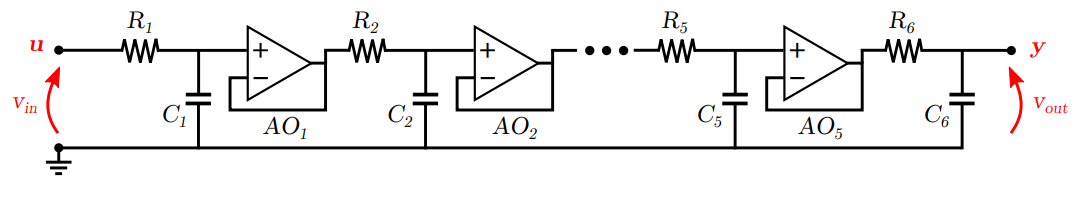
\includegraphics[width=0.43\textwidth]{./IMAGENES/diag_placa.png}
  \caption{Esquemático de la placa}
  \label{fig:placa}
\end{figure}

\subsection{Respuesta al escalón}
Se empleó una señal PWM con ciclo de trabajo del $20\%$, para hacer que la entrada vaya de 0V a 1V (en el segundo 0), luego de que se estableciera la salida (a los 3 segundos), se cambió el PWM al $80\%$ de manera que actuará como escalón, y luego de pasados 3 segundos, se volvió a llevar el ciclo de trabajo al $20\%$. Esto se realizó tanto en simulación (en Proteus), como en la placa física, como los datos son idénticos para ambos casos, de ahora en adelante se referirá solamente a los datos.

\begin{figure}[H]
  \centering
  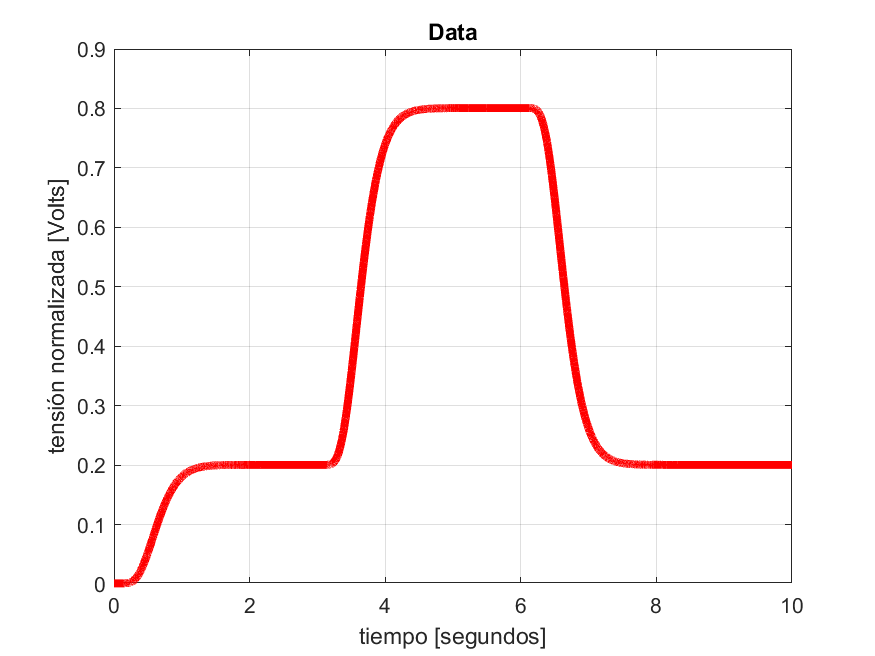
\includegraphics[width=0.43\textwidth]{./imagenes/datos_resp_escalon.png}
  \caption{Respuesta al escalón del sistema (\textit{normalizada a 5V})}
  \label{fig:resp_esc}
\end{figure}

\subsection{Modelos de la planta}
Una vez hecho el relevamiento de los datos, se emplearon para obtener un modelo de la planta original de alto orden, uno del tipo FOPDT\footnote{First order plus dead time: primer orden más tiempo muerto} y otro SOPDT\footnote{Second order plus dead time: segundo orden más tiempo muerto}, para esto utilizamos la aplicación de Matlab System Identification\footnote{Herramiento de MATLAB Toolbox que permite hacer identificación de sistemas} habiendo previamente procesados los datos (se tuvo que linealizar el tiempo).

\subsubsection{Modelo FOPDT}
\begin{equation}
  \frac{e^{-0.33791s}}{0.28802s+1}
\end{equation}

\subsubsection{Modelo SOPDT}
\begin{equation}
  \frac{e^{-0.24087}}{(0.18561+1)(0.18561+1)}
\end{equation}

\subsubsection{Modelo de orden 6}
\begin{equation}
  \tiny{\frac{1.261*10^6}{s^6+75.11s^5+1869s^4+2.523104s^3+1.888105s^2+7.568105s^+1.26106}}
\end{equation}

\vspace{1em}

\subsubsection{Precisión de los modelos}


\begin{table}[H]
\centering
\begin{tabular}{|l|c|c|c|}
\hline
\textbf{Tipo} & \multicolumn{1}{l|}{\textbf{EFP}}     & \multicolumn{1}{l|}{\textbf{EMC}}     & \multicolumn{1}{l|}{\textbf{fit porcentual}} \\ \hline
FOPDT   & 0.001008                     & 0.01007                      & 91.97\%                             \\ \hline
SOPDT   & 0.0002428                    & 0.0002421                    & 96.06\%                             \\ \hline
Orden 6 & $3.963*10^{-9}$ & $3.912*10^{-9}$ & $99.98\%$                             \\ \hline
\end{tabular}
  \caption{Precisión de los modelos}
  \label{tab:precision_modelos}
\end{table}

Es importante tener en cuenta que estos modelos están \textbf{normalizados} con respecto a 5V. \\

\textit{Para corroborar la precisión de los modelos, se obtuvieron más datos con otro escalón, con los que se hicieron las verificaciones y cálculos.}
Los resultados de estos modelos se presentan en la figura \ref{fig:resp_esc_modelos}, para hacer una mejor interpretación de los datos y los modelos, se centró la respuesta al escalón de los datos entre 1V y 4V, y entre 3 y 6 segundos.

\begin{figure}[H]
  \centering
  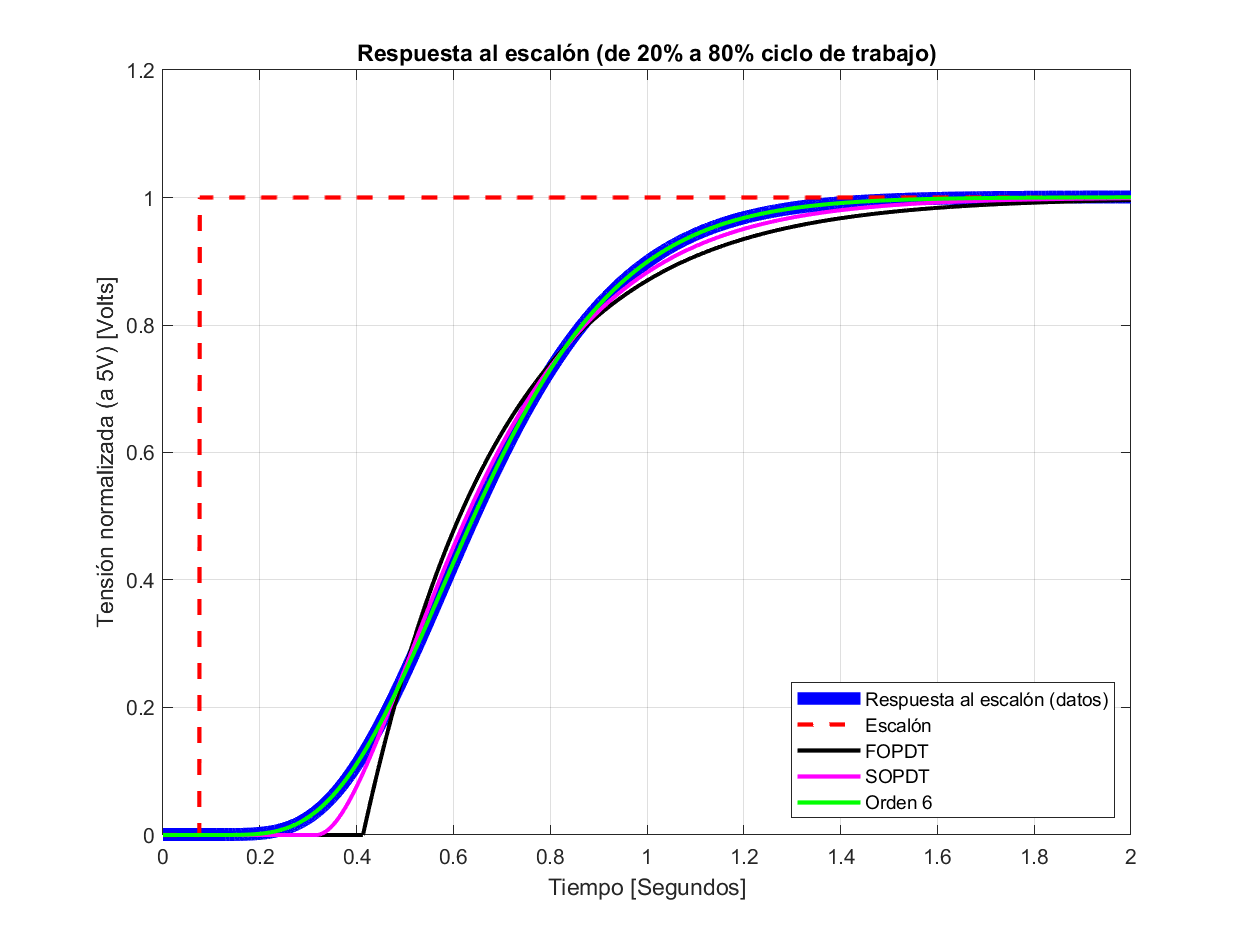
\includegraphics[width=0.43\textwidth]{./IMAGENES/resp_esc.png}
  \caption{Respuesta al escalón de los modelos}
  \label{fig:resp_esc_modelos}
\end{figure}

\subsubsection{Familia de plantas}

Considerando una tolerancia de los elementos del circuito de un $10\%$ (al ser el producto de estos, termina siendo la suma, es decir una tolerancia del $20\%$) y partiendo del modelo de orden 6, es posible establecer una familia de modelos a partir de un peso de incertidumbre dinámica global. Se consideró un peso de \textbf{incertidumbre aditiva}, ya que el mismo es el más adecuado a la hora de aproximar un modelo de orden elevado con otro de orden reducido. La condición a evaluar para el diseño del peso es la siguiente:

\begin{equation*}
  |G(jw) - G_0(jw)| < |W\delta(jw)|
\end{equation*}

Donde G es la familia de plantas y $G_0$ se obtiene a partir del modelo FOPDT obtenido. Entonces graficando esta condición para distintos valores para la constante de tiempo de G se obtuvo la siguiente función peso, compuesta de un cero y un polo:

\begin{equation*}
  G_0 = \frac{e^{-0.33791s}}{0.28802s+1}
\end{equation*}

\begin{equation*}
  W_a = \frac{0.2s}{0.4s+1}
\end{equation*}

De manera tal que nuestra familia de plantas queda de la siguiente forma

\begin{equation*}
  G(s) = g_0 + (1 + W_{a}\delta)  \hspace{1em},\hspace{1em} |\delta| \leq 1
\end{equation*}
\begin{equation*}
  G(s) = \frac{e^{-0.33791s}}{0.28802s+1} + (1 + \frac{0.2s}{0.4s+1)}\delta) \hspace{1em},\hspace{1em} |\delta| \leq 1
\end{equation*}

\begin{figure}[H]
  \centering
  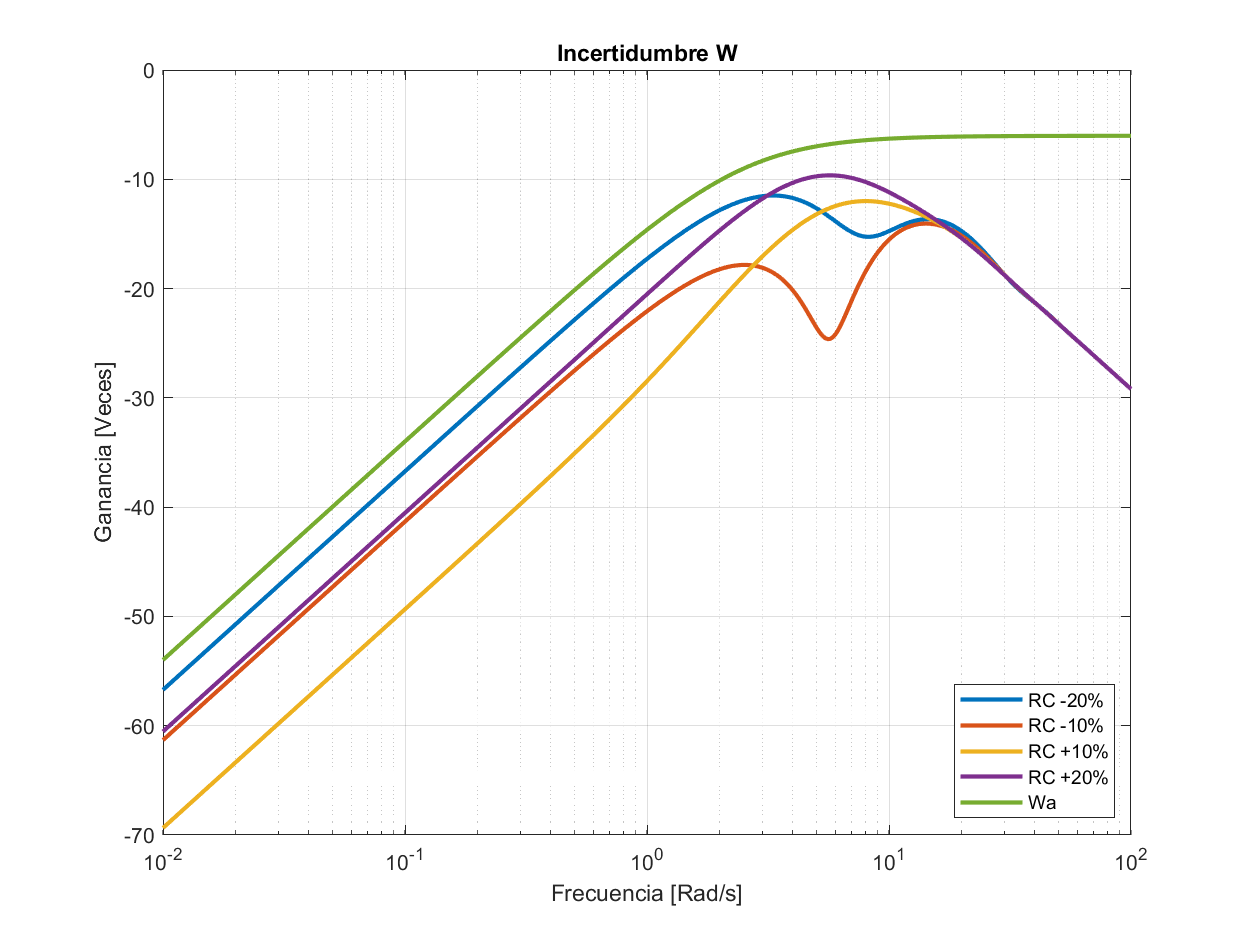
\includegraphics[width=0.43\textwidth]{./IMAGENES/wa.png}
  \caption{Incertidumbre y modelo $W_a$}
  \label{fig:incertidumbres}
\end{figure}

\subsection{Señal pseudoaleatoria}

Se empleó una señal pseudoaleatoria como entrada al sistema para hacer la identificación del mismo. Se tomó como periodo de la señal $T_{PRBS} = 200ms$ y una cantidad de bits $N=7$, con esto se tiene un tiempo de ensayo $D_s = 25.4$. Estos valores cumplen con la frecuencia de \textit{Nyquist} y el tiempo de \textit{rising} del sistema $t_{r} \cong 1.4segundos$ (ancho de banda $BW = \frac{1}{t_{r}} \cong 0.71Hz$).
\textit{Nuevamente las tensiones se normalizaron con respecto a 5V.}

\begin{figure}[H]
  \centering
  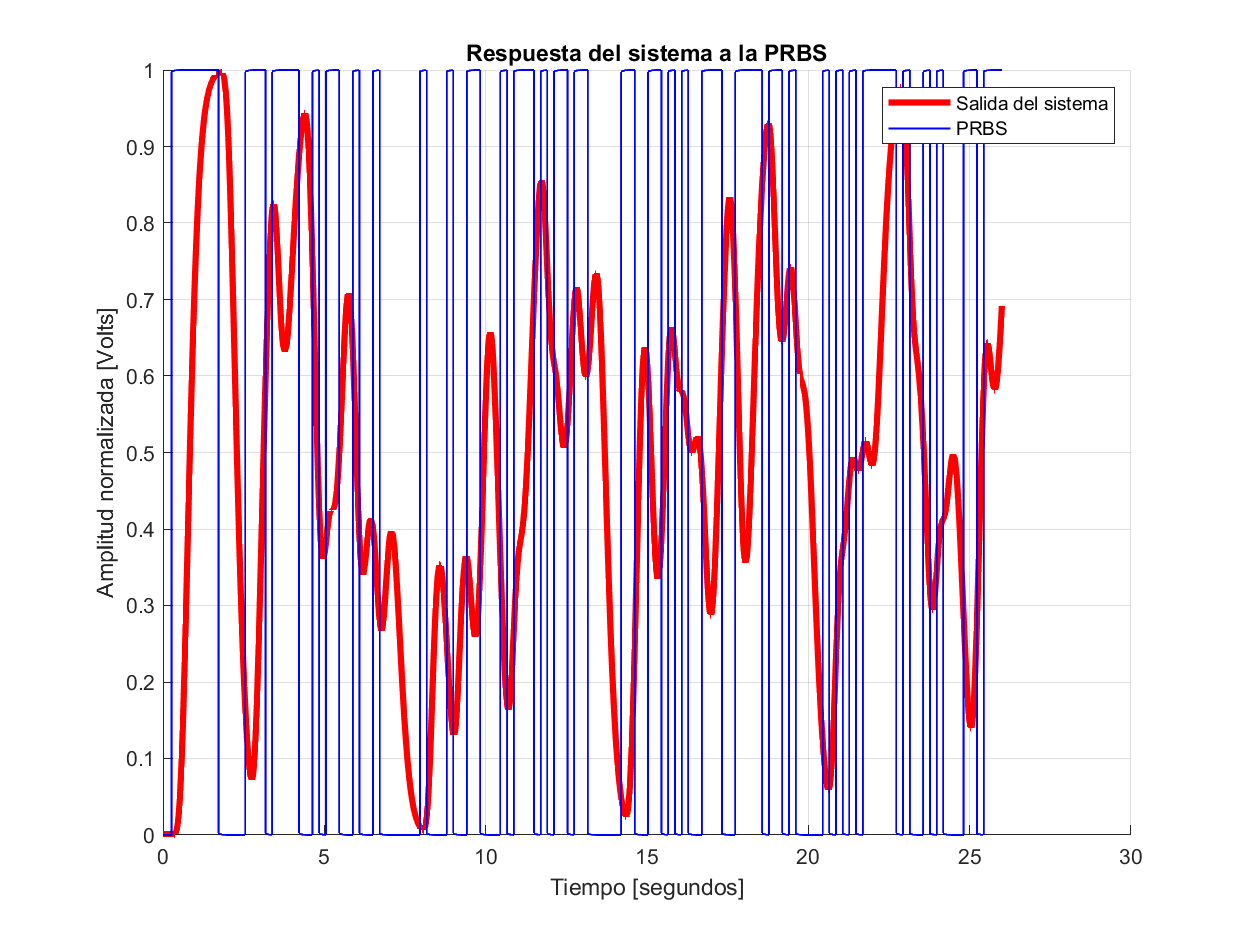
\includegraphics[width=0.43\textwidth]{./IMAGENES/datos_prbs.png}
  \caption{Respuesta del sistema a la PRBS}
  \label{fig:datos_prbs}
\end{figure}

Luego se empleó la herramienta \textit{System Identification} para obtener los mismos modelos que antes. Los modelos obtenidos se muestran a continuación y, como se puede observar, son mucho peor que los primeros.

\subsubsection{Modelo FOPDT}
\begin{equation}
  \frac{e^{-0.2948s}}{0.3772s+1}
\end{equation}

\subsubsection{Modelo SOPDT}
\begin{equation}
  \frac{e^{-0.20498}}{(0.20383+1)(0.20383+1)}
\end{equation}

\subsubsection{Modelo de orden 6}
\begin{equation}
  \tiny{\frac{1.261*10^6}{s^6 + 2.652 s^5 + 109 s^4 + 209.1 s^3 + 3777 s^2 + 4121 s + 4.084*10^{4}}}
\end{equation}

\begin{table}[H]
\centering
\begin{tabular}{|l|c|c|c|}
\hline
\textbf{Tipo} & \multicolumn{1}{l|}{\textbf{EFP}}     & \multicolumn{1}{l|}{\textbf{EMC}}     & \multicolumn{1}{l|}{\textbf{fit porcentual}} \\ \hline
FOPDT   & 0.01969                     & 0.01962                      & $42.74\%$                             \\ \hline
SOPDT   & 0.01656                     & 0.01648                      & $47.53\%$                            \\ \hline
Orden 6 & 0.3103                      & 0.0001459                    & $50.2\%$                             \\ \hline
\end{tabular}
  \caption{Precisión de los modelos}
  \label{tab:precision_modelos_prbs}
\end{table}

\section{Diseño de controlador PID}
En la siguiente sección se presenta el diseño de un controlador del tipo PID de la planta mostrada en la primer sección, haciendo énfasis en la teoría de controladores PID en sistemas con Retardo. Dicho Controlador fue implementado en un microcontrolador ATMega328p sobre el cual se efectuaron ensayos de forma experimental de forma física y virtual a través de la herramienta de software Proteus 8 Professional.
Para el diseño del mismo se utilizó el modelo de primer orden obtenido en la primer sección:

\begin{equation*}
  G_1(s) = \frac{e^{(-0.33791s)}}{0.28802s+1}
\end{equation*}

\subsection{PID con predictor Smith}
Se parte del diseño de un controlador PI aplicado a la planta definida como:

\begin{equation*}
  P_n(s) = \frac{K_{p}e^{-Ls}}{Ts+1}
\end{equation*}

\begin{equation*}
  G_n(s) = \frac{K_{p}}{Ts+1}
\end{equation*}

\begin{equation*}
  C(s) = \frac{K_{1}(T_{1}s+1)}{T_{1}}
\end{equation*}

Al sintonizar el sistema para cancelar el polo del modelo de lazo abierto, se obtiene el controlador equivalente:

\begin{equation*}
  C_{e}(s) = \frac{K_{1}(Ts+1)}{Ts+K_{1}K_{p}(1-e^{-Ls})}
\end{equation*}

Usando una aproximación de Padé de primer orden para el retardo y equiparando a un controlador PID en formato serie con filtrado en la acción derivativa, se obtiene:

\begin{equation*}
  C_{e}(s) = \frac{K_{c}(T_{I}s+1)(T_{D}s+1)}{T_{I}s(1+\alpha T_{D}s)}
\end{equation*}

\begin{equation*}
  \alpha = \frac{1}{1+\frac{L}{T_{0}}}
\end{equation*}

\begin{equation*}
  K_c = \frac{T}{(L+T_{0})K_p}
\end{equation*}

 Siendo el valor de $K_{p}$ es la ganancia de la planta, L es el retardo y $T_{I}$ es la constante de tiempo, por lo tanto solo se tendrá que sintonizar el valor de $T_{0}$. \\
Para la sintonización de $T_0$, se diseña el sistema en Simulink\footnote{Herramienta provista en el Toolbox de MATLAB.}. Se evalúa la respuesta al escalón considerando una perturbación también en escalón, aplicada a los 5 segundos. \\
Primero probamos con un valor pequeño de T0=0.1, donde se observa un sobrepeso significativo en la respuesta (línea amarilla), aunque la perturbación se rechaza. Sin embargo, la acción de control (línea verde) resulta excesiva, dificultando su implementación en un Arduino.\\

\begin{figure}[H]
  \centering
  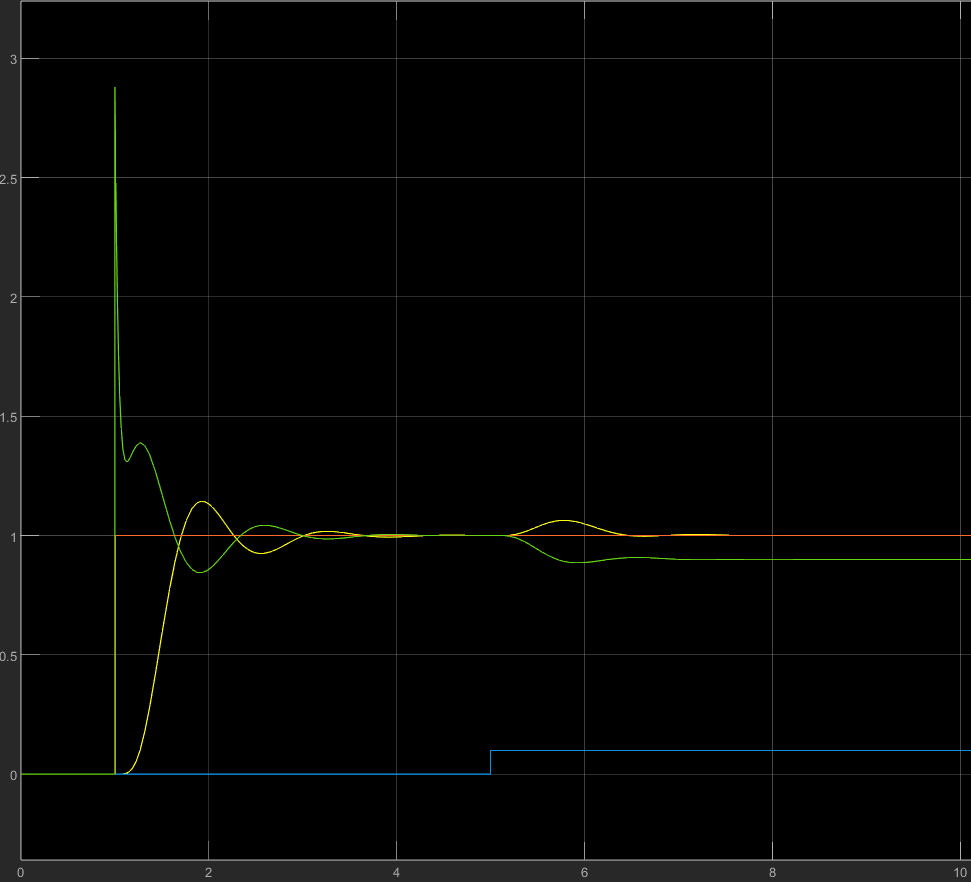
\includegraphics[width=0.43\textwidth]{./IMAGENES/pid1.png}
  \caption{Simulación en Simulink \(T_{0} = 0.1\)}
  \label{fig:pid1}
\end{figure}

\begin{figure}[H]
  \centering
  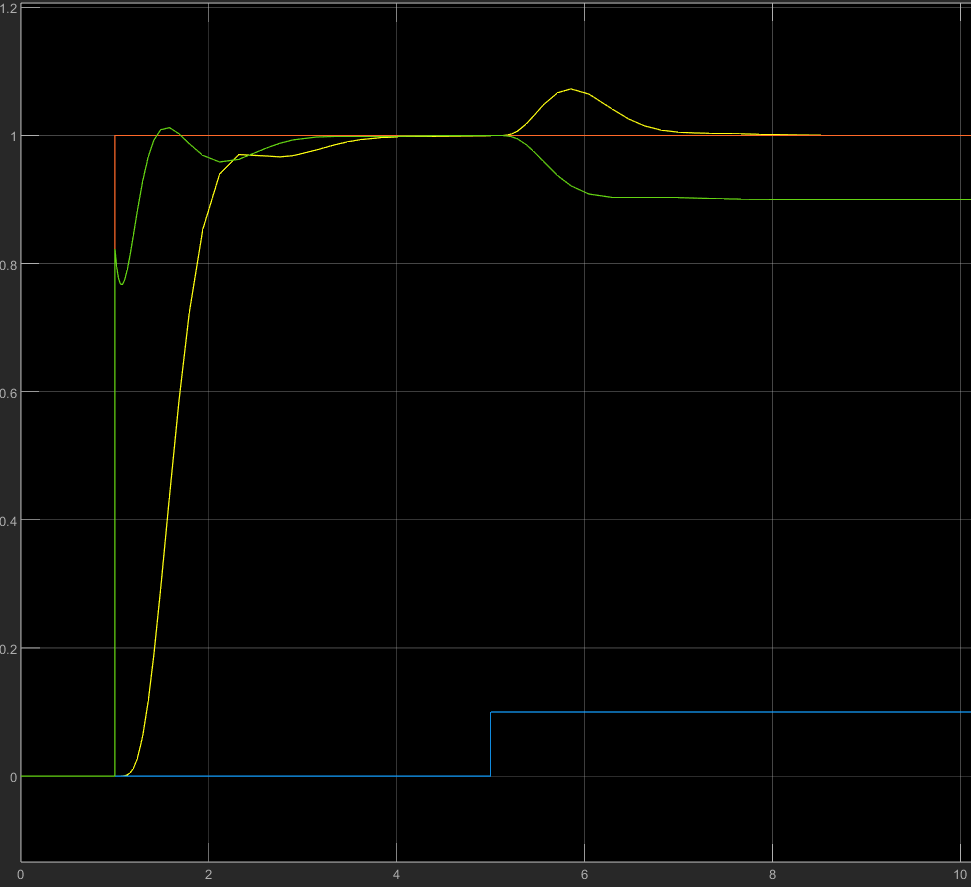
\includegraphics[width=0.43\textwidth]{./IMAGENES/pid2.png}
  \caption{Simulación en Simulink \(T_{0} = 0.35\)}
  \label{fig:pid2}
\end{figure}

Aumentando el valor de $T_{0}$ a 0.35, se puede observar que con este ajuste, el sobrepaso desaparece, pero la magnitud de la acción de control sigue siendo alta.Aunque hay que aclarar que el rechazo a la perturbación, debido a la cancelación del polo dominante del sistema, que aparece en la transferencia entre la perturbación y la salida, no se podrá rechazar más rápido que la constante de tiempo de la planta.

\subsection{Filtro}

Para reducir la acción de control y mejorar la velocidad de respuesta sin sobrepaso, se implementa un filtro en la entrada de la referencia. El filtro usado es el siguiente:

\begin{equation*}
  F(s) = \frac{(1+\beta T_{r}s)}{(1+T_{r}s)}
\end{equation*}

El filtro se conecta en serie con la referencia, como se muestra en el diagrama correspondiente:

\begin{figure}[H]
  \centering
  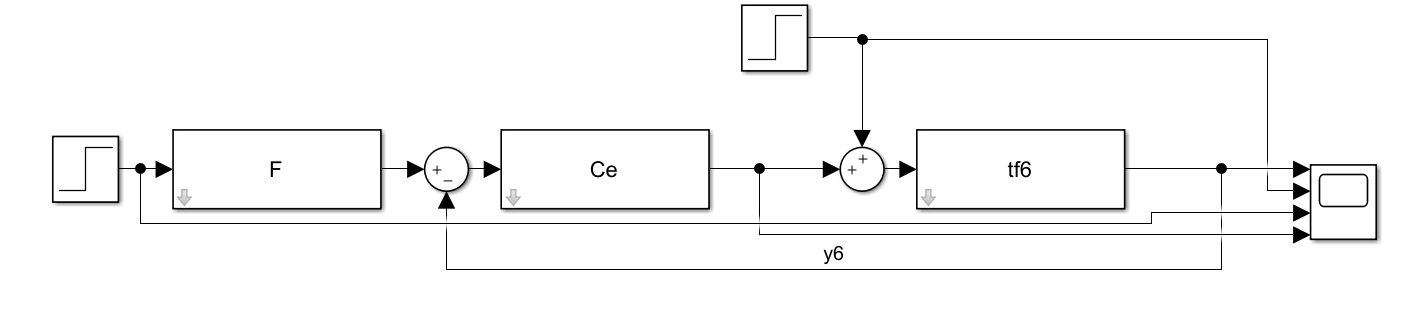
\includegraphics[width=0.43\textwidth]{./IMAGENES/pid3.png}
  \caption{Diagrama en bloques del sistema en Simulink}
  \label{fig:pid3}
\end{figure}

Al simular nuevamente con $T_{0}=0.35$, observamos que los picos de la acción de control disminuyen significativamente, lo que indica una mejora en la respuesta. Sin embargo, para garantizar un rango de seguridad adicional y evitar riesgos de inestabilidad o sobrecarga del controlador, se decidió incrementar ligeramente el valor de $T_{0}=0.35$.


\begin{figure}[H]
  \centering
  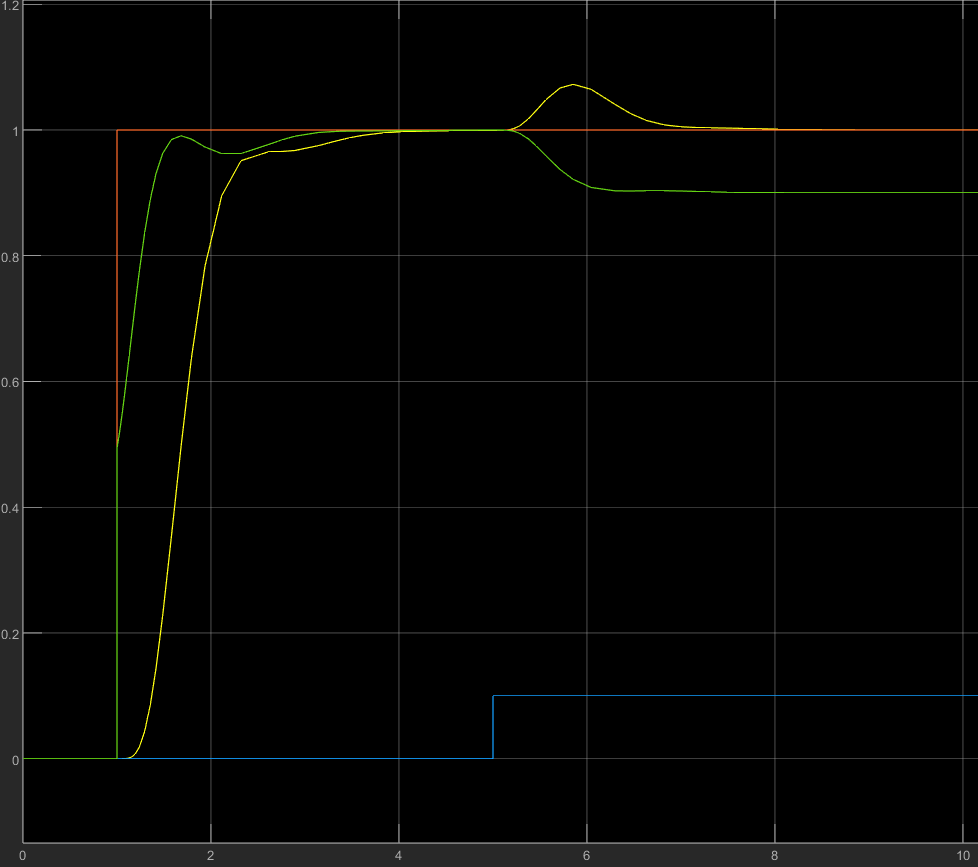
\includegraphics[width=0.43\textwidth]{./IMAGENES/pid4.png}
  \caption{Simulación en Simulink \(T_{0} = 0.35\)}
  \label{fig:pid4}
\end{figure}

\begin{figure}[H]
  \centering
  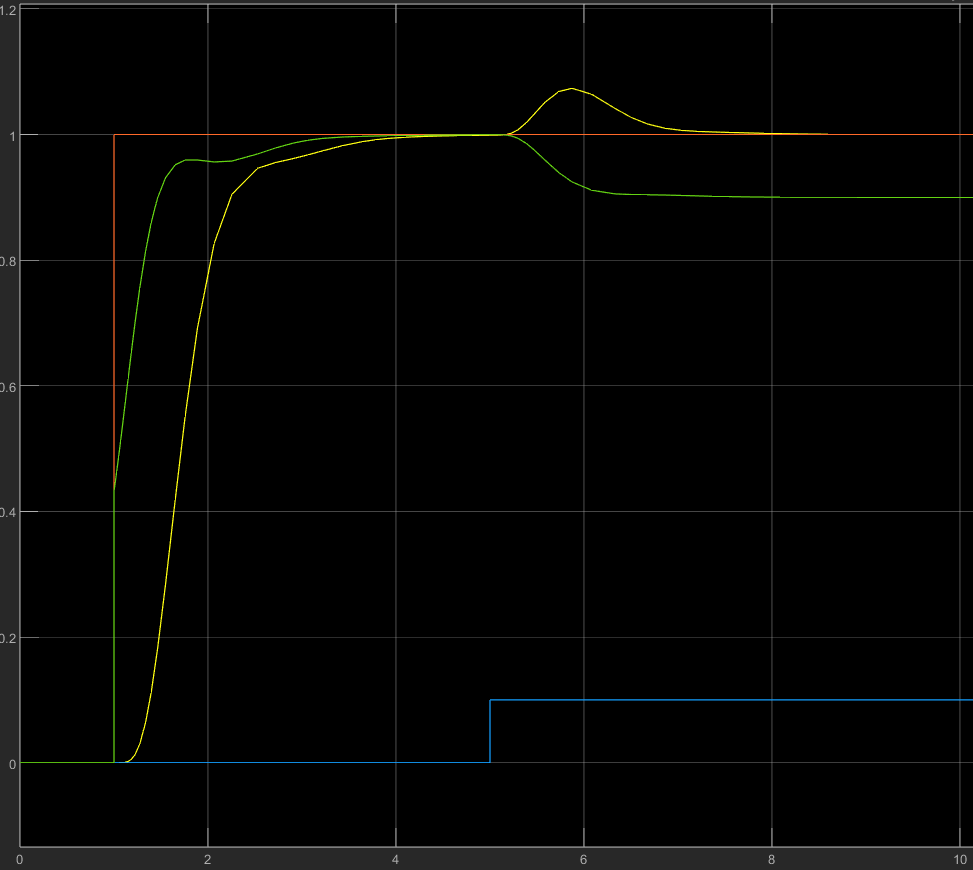
\includegraphics[width=0.43\textwidth]{./IMAGENES/pid5.png}
  \caption{Simulación en Simulink \(T_{0} = 0.4\)}
  \label{fig:pid5}
\end{figure}

Con $T_{0}=0.4$, la acción de control no presenta picos significativos, lo que permite implementarla en un Arduino sin problemas. Además, el rechazo a la perturbación es suficientemente rápido, con el pico ocurriendo entre 5.2 y 5.7 segundos, es decir, un tiempo de 0.5 segundos.

Dado que la constante de tiempo de la planta es T=0.28 segundos, este tiempo de rechazo es adecuado, ya que no puede ser inferior debido a la cancelación del polo dominante del sistema. Reducir aún más $T_{0}$ podría hacer la acción de control demasiado agresiva, generando sobrepasos u oscilaciones. Por lo tanto, $T_{0}=0.4$ es un valor equilibrado para cumplir con los requisitos del diseño.

\subsection{Comprobación de robustez}

El controlador diseñado demostró cumplir de forma satisfactoria con las especificaciones de diseño para el modelo estimativo de la planta. Sin embargo, es necesario establecer un peso de incertidumbre adecuado para representar el error de modelado presente. Considerando el peso de incertidumbre aditiva propuesto en la sección anterior, se obtiene que la condición necesaria para asegurar robustez es la siguiente:

\begin{equation*}
  |C(jw)W(jw)| < |1 + C(jw)G_{0}(jw)|
\end{equation*}
En la siguiente gráfica se puede evaluar esta condición para el controlador diseñado.

\begin{figure}[H]
  \centering
  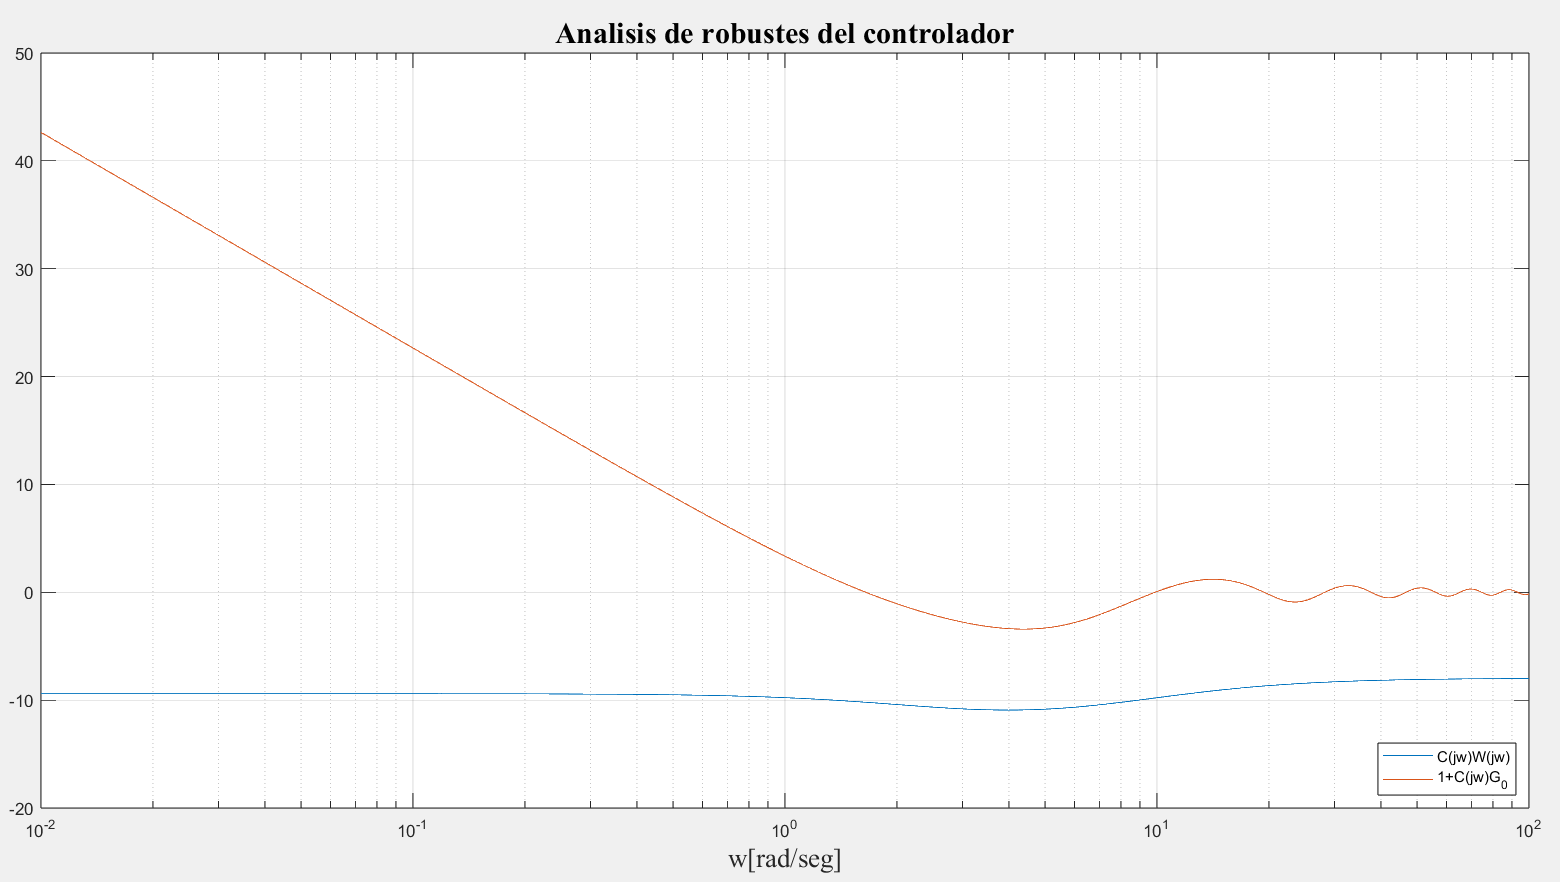
\includegraphics[width=0.43\textwidth]{./IMAGENES/pid6.png}
  \caption{Comprobación de condición de robustez}
  \label{fig:pid6}
\end{figure}

En la gráfica de validación, se observa que esta condición se cumple, garantizando robustez en el diseño.

\subsection{Discretización y simulación}

Por último, se desarrolló un código en Arduino para implementar el controlador discreto. Para ello, se emplearon aproximaciones numéricas tanto para la derivada como para la integral.
Una vez sintonizado el modelo PID en formato serie, se convirtió el controlador al formato paralelo antes de realizar la discretización. Esto se realizó porque trabajar con las ecuaciones en formato paralelo resulta más conveniente y práctico para este propósito.

\begin{equation*}
  C_{e}(s) = \frac{(K_p + \frac{K_I}{s} + K_{D}s)}{(1 + sT_{f})}
\end{equation*}

Donde:

\begin{equation*}
  T_{f} = 0.5 * \alpha * L
\end{equation*}

\begin{equation*}
  K_{I} = \frac{K_c}{T_I}
\end{equation*}

\begin{equation*}
  K_D = 0.5*L*K_{c}
\end{equation*}

\begin{equation*}
  K_p = Kc\frac{(T + 0.5*L)}{T}
\end{equation*}

Partiendo de la relación entre la salida de la acción de control U(s) y el error E(s):

\begin{equation*}
  U(s) = \frac{K_{p} + K_{I} + K_{D}s}{1+sT_{f}} E(s)
\end{equation*}

Al aplicar la transformada inversa de Laplace y despejar, se obtiene la siguiente ecuación diferencial, que será la base para la discretización:

\begin{equation*}
  u(t) + T_{f} u'(t) = K_{p} e(t) + K_{I} \int e(t)dt + K_{D} e'(t)
\end{equation*}

A partir de esta expresión, se discretizan los términos de la siguiente manera:
Término proporcional (P):

\begin{equation*}
  P = K_{p} e(t) \rightarrow P[k] = K_{p} e[k]
\end{equation*}

Término derivado asociado a la salida (D1):

\begin{equation*}
  D1 = T_{f} u'(t) \rightarrow D1[k] = T_{f} \frac{( u[k] - u[k-1] )}{h}
\end{equation*}

Término integral (I):

\begin{equation*}
  I = K_{I} \int  e(t)dt \rightarrow I' = K_{I} e \rightarrow I[k+1] = h*K_{I}e[k] + I[k]
\end{equation*}

Término derivado asociado al error (D2):

\begin{equation*}
  D2 = K_{D} e'(t) \rightarrow D2[k] = K_{D} \frac{( e[k] - e[k-1] )}{h}
\end{equation*}

Sumando todos los términos, se obtiene la ecuación en diferencias que describe el controlador discreto:

\begin{equation*}
  u[k] = \frac{(e[k](K_{p} + \frac{K_{D}}{h}) - e[k-1]\frac{K_{D}}{h} + I[k] + \frac{T_{f}}{h} * u[k-1])}{1 + \frac{T_{f}}{h}}
\end{equation*}

Esta ecuación fue implementada en el código de Arduino. 
Antes de programar el controlador en el microcontrolador, se realizó una simulación en Proteus para verificar su correcto funcionamiento. A continuación, se muestra una imagen de la simulación realizada:

\begin{figure}[H]
  \centering
  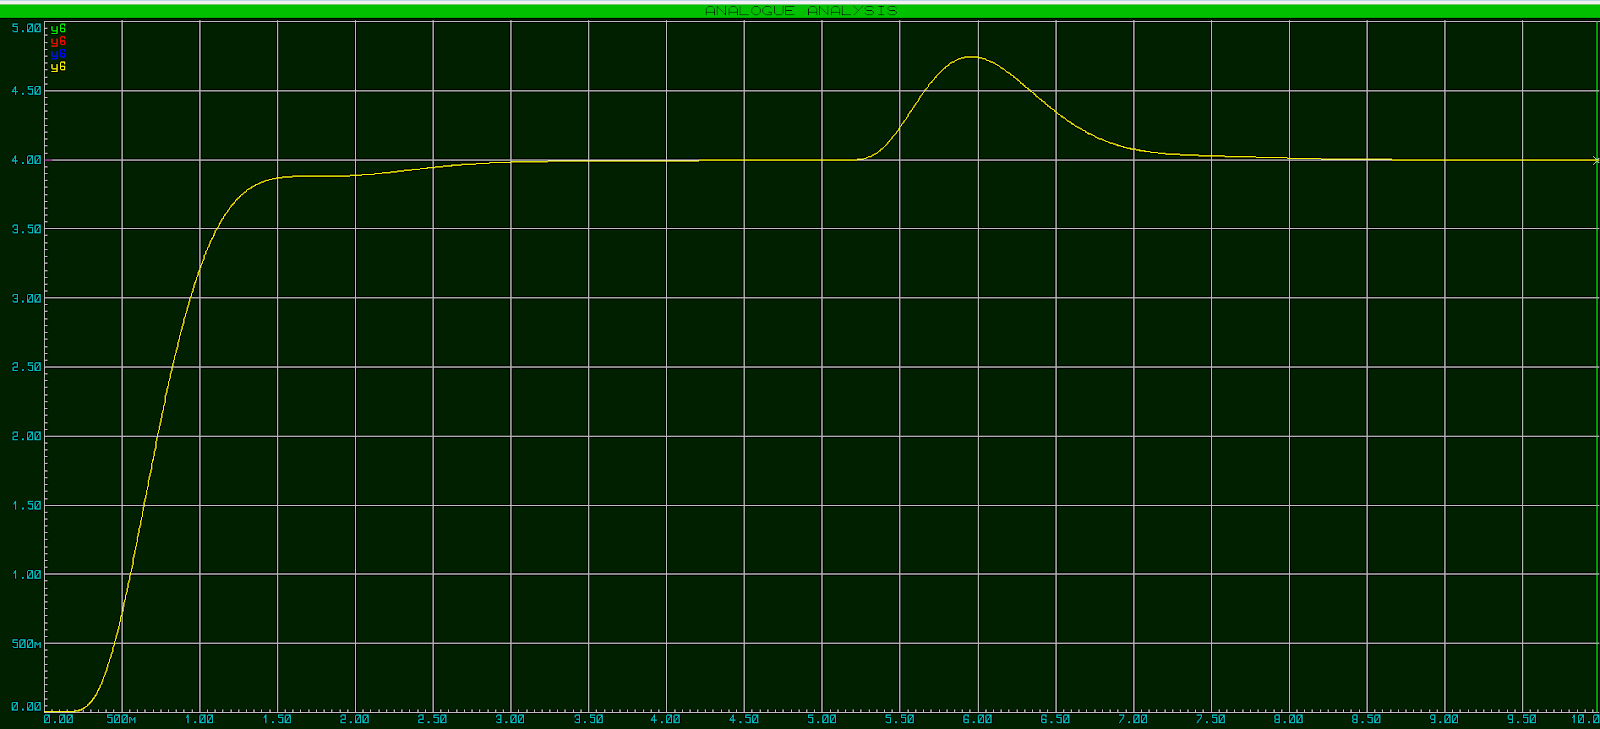
\includegraphics[width=0.43\textwidth]{./IMAGENES/pid7.png}
  \caption{Simulación en Proteus}
  \label{fig:pid7}
\end{figure}

\subsection{Ensayo experimental}

Finalmente el programa fue cargado en un Arduino UNO, obteniéndose resultados experimentales consistentes con las simulaciones en MATLAB y Proteus, validando la correcta implementación y sintonización.

\begin{figure}[H]
  \centering
  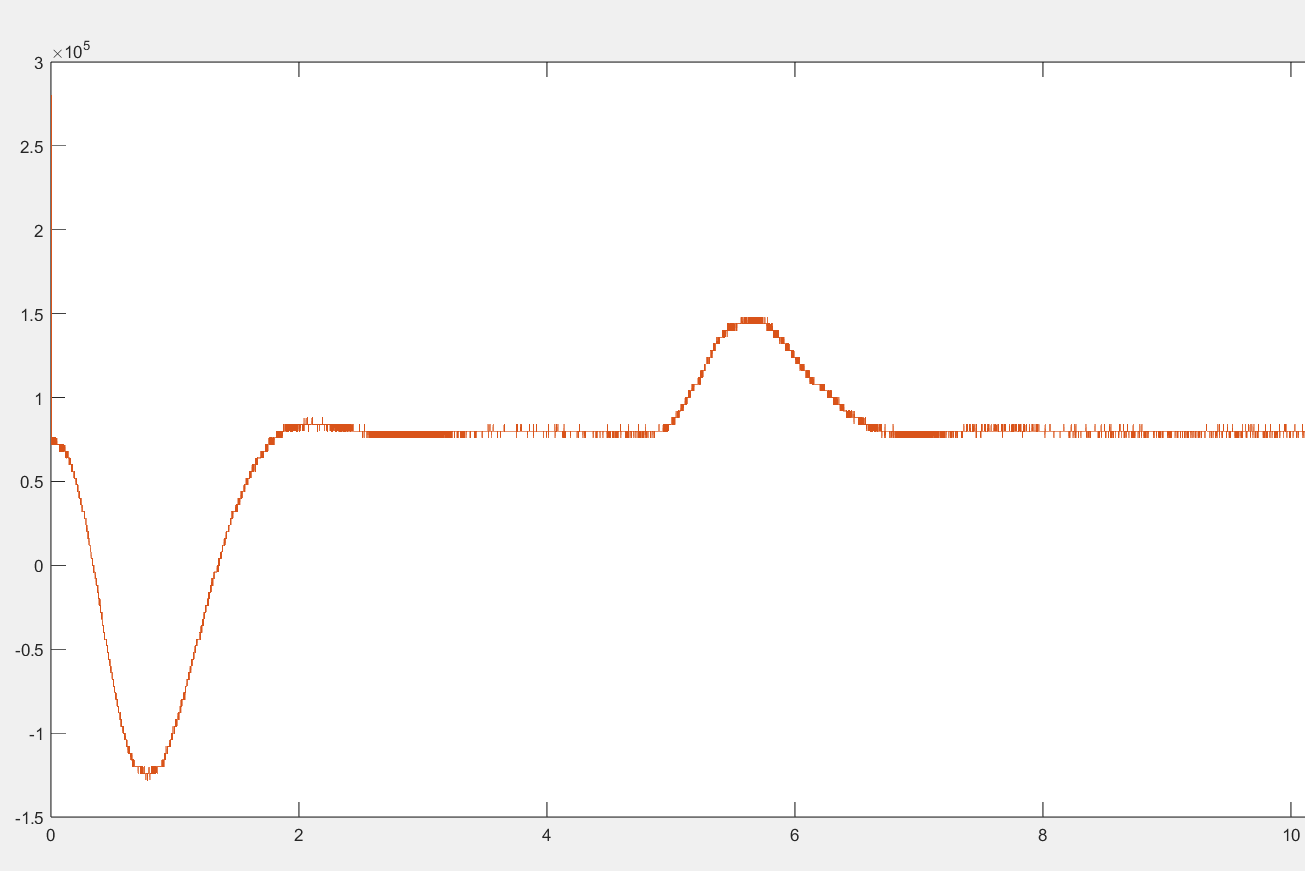
\includegraphics[width=0.43\textwidth]{./IMAGENES/pid8.png}
  \caption{Resultado experimental}
  \label{fig:pid8}
\end{figure}

\section{Conclusión}

La realización del trabajo permitió abordar de manera integral las etapas clave de un proyecto de control automático, desde la identificación precisa del sistema hasta el diseño y validación experimental de un controlador PID. A través del uso de herramientas como MATLAB, Simulink, Proteus y Arduino, se lograron modelos ajustados a diferentes niveles de precisión y se implementaron estrategias robustas que cumplen con los requisitos de diseño y operan adecuadamente en un entorno físico. Los resultados experimentales y simulados fueron consistentes, validando la metodología empleada y destacando la importancia de la sintonización cuidadosa y la consideración de incertidumbres en sistemas reales.

\end{document}